\subsection{Privilege Level Switching}
\label{sec:faults}

Applications software needs a method to invoke the kernel, because it cannot
perform privileged operations, such as network or disk I/O. At the same time,
ring 3 software cannot be offered the ability to jump arbitrarily into kernel
code, because that would compromise the kernel's ability to isolate
applications and enforce security invariants.\footnote{For example, when an
application wishes to write a file to the disk, the kernel must check if the
application's user has access to that file. If the ring 3 code could perform an
arbitrary jump in kernel space, it would be able to skip the access check.}
Therefore, the processor has designated methods for switching privilege levels,
which protect the integrity of the privileged software.

This section describes the privilege switching mechanisms that impact the SGX
design, summarized in Figure~\ref{fig:cpu_ring_switch}. Also, understanding the
considerations behind privilege switching is useful when analyzing SGX, because
the process of calling code inside an enclave is similar to switching privilege
levels, as an enclave's code must be able to enforce its own security
invariants, just like an OS kernel.

% Fast System Calls in 64-Bit Mode: SDM S 5.8.8
% Architectural MSRs: SDM S 35.1

\begin{figure}[hbt]
  \center{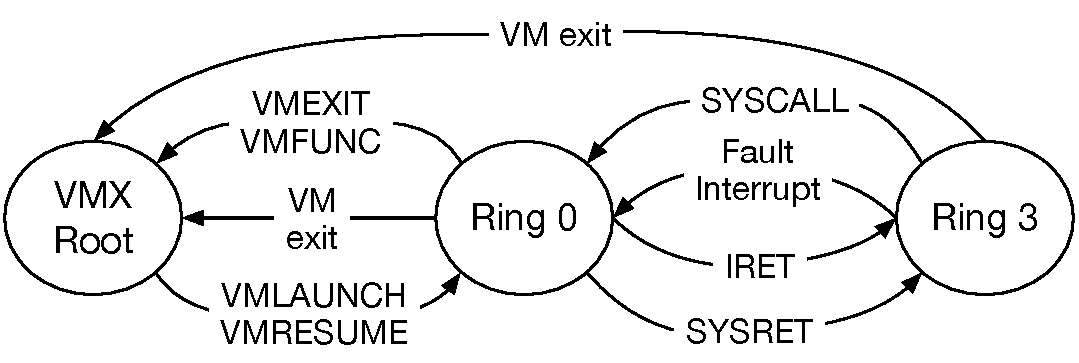
\includegraphics[width=85mm]{figures/cpu_ring_switch.pdf}}
  \caption{
    Modern privilege switching methods in the 64-bit Intel architecture.
  }
  \label{fig:cpu_ring_switch}
\end{figure}

On modern processors, application software uses the SYSCALL instruction to
invoke ring 0 code, and the kernel uses SYSRET to switch the privilege level
back to ring 3. SYSCALL jumps into a predefined kernel location, which is
specified by writing to \textit{architectural\footnote{Despite the
``model-specific'' in MSR, \textit{architectural} MSRs are a part of the Intel
architecture, and their semantics are stable across processor generations.}
Model Specific Registers (MSRs)}. MSRs can only be read or written by ring 0
code, therefore application softeware cannot execute arbitrary kernel code.
The SYSRET instruction switches back to ring 3 and jumps to the address in RCX,
which is set by the SYSCALL instruction. The SYSCALL / SYSRET pair is optimized
for speed by avoiding any memory references. The design can get away without a
stack because kernel calls are not recursive.

% Interrupt and Exception Handling: SDM S 6.1, S 6.2
% Access Rights: SDM S 4.6
% Page-Fault Exceptions: SDM S 4.7

The processor also performs a switch from ring 3 to ring 0 when a \textit{
hardware exception} occurs while executing application code. Some exceptions
indicate bugs in the application, whereas other exceptions require kernel
action. A \textit{general protection fault} (\#GP) occurs when software
attempts to perform a disallowed action, such as setting the CR3 register from
ring 3. A \textit{page fault} (\#PF) occurs when address translation encounters
a page table entry whose P flag is 0, or attempting to use a page in a way
inconsistent with the access bits in its page table entry, for example
accessing a page whose S bit is set from ring 3.

% Interrupt Descriptor Table (IDT): SDM S 6.10

When a hardware exception occurs in application code, the CPU performs a ring
switch, and calls the corresponding \textit{exception handler}. For example,
the \#GP handler typically terminates the application's process, while the \#PF
handler reads the swapped out page back into RAM and resumes the application's
execution.

The exception handlers are a part of the OS kernel, and their locations are
specified in the first 32 entries of the Interrupt Descriptor Table (IDT),
whose structure is shown in Table~\ref{fig:idt_entry}. The IDT's physical
address is stored in the IDTR register, which can only be accessed by ring 0
code. Kernels protect the IDT memory using page tables, so that ring 3 software
cannot access it.

\begin{table}[hbt]
  \center{\begin{tabular}{| l | r |}
  \hline
  \textbf{Field} & \textbf{Bits} \\
  \hline
  Handler RIP & 64 \\
  \hline
  Handler CS & 16 \\
  \hline
  Interrupt Stack Table (IST) index & 3 \\
  \hline
  \end{tabular}}
  \caption{
    The essential fields of an IDT entry in 64-bit mode. Each entry points to a
    hardware exception or interrupt handler.
  }
  \label{fig:idt_entry}
\end{table}

Each IDT entry has a 3-bit index pointing into the Interrupt Stack Table (IST),
which is an array of 8 stack pointers stored in the TSS described in
\S~\ref{sec:segments}.

% 64-Bit Mode Stack Frame: SDM S 6.14.2
% IRET in IA-32e Mode: SDM S 6.14.3
% Stack Switching in IA-32e Mode: SDM S 6.14.4
% Interrupt Stack Table: SDM S 6.14.5

When a hardware exception occurs, the execution state may be corrupted, and the
current stack cannot be relied on. Therefore, the CPU first uses the handler's
IDT entry to set up a known good stack. SS is loaded with a null descriptor,
and RSP is set to the IST value pointed by the IDT entry. After switching to a
reliable stack, the CPU pushes the snapshot in Table~\ref{fig:fault_stack} on
the stack, then loads the IDT entry's values into the CS and RIP registers,
which trigger the execution of the exception handler.

\begin{table}[hbt]
  \center{\begin{tabular}{| l | r |}
  \hline
  \textbf{Field} & \textbf{Bits} \\
  \hline
  Exception SS & 64 \\
  \hline
  Exception RSP & 64 \\
  \hline
  RFLAGS & 64 \\
  \hline
  Exception CS & 64 \\
  \hline
  Exception RIP & 64 \\
  \hline
  Exception code & 64 \\
  \hline
  \end{tabular}}
  \caption{
    The snapshot pushed on the handler's stack when a hardware exception
    occurs. IRET restores registers from this snapshot.
  }
  \label{fig:fault_stack}
\end{table}

After the exception handler completes, it uses the \texttt{IRET} (interrupt
return) instruction to load the registers from the on-stack snapshot and switch
back to ring 3.



If an EPT entry has the P flag set to 0, the CPU performs a VM exit, and the
hypervisor has an opportunity to bring the page into RAM.





